\subsection{Angular distribution and observables}
\label{sec:kpimm:angular-distribution}

The final state of the decay \BdToKpimm can be fully described by five kinematic variables: three decay angles (\ctl, \ctk, $\phi$) and two masses; \mkpi, the invariant mass of the \kaon\pion system and \qsq, the invariant mass squared of the dimuon system. Each of the decay angles are shown schematically in Fig.~\ref{fig:kpimm:angles}. The angle \thetal is defined as the angle between the direction of the \mup (\mun) in the dimuon rest frame and the direction of the dimuon in the \Bz (\Bzb) rest frame. The angle \thetak is defined as the angle between the direction of the kaon in the \KstarJ (\KstarJb) rest frame and the direction of the \KstarJ (\KstarJb) in the \Bz (\Bzb) rest frame. The angle $\phi$ is the angle between the plane containing the \mup and \mun and the plane containing the kaon and pion. The explicit definitions of each of the angles can be found in~\cite{kstmm-1fb}.

\begin{figure}[!htb]
  \centering
  \resizebox{\columnwidth}{!}{
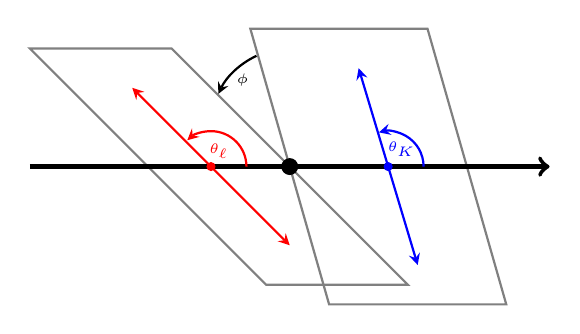
\begin{tikzpicture}
  %\draw[step=1cm,gray,very thin] (0,0) grid (7,4);
  %planes
  \draw[thick,gray] (0.2,3.5)--(2,3.5)--(5,0.5)--(3.2,0.5)--cycle;
  \draw[thick,gray] (3.,3.75)--(4.,0.25)--(6.25,0.25)--(5.25,3.75)--cycle;
  %axis
  \draw[ultra thick,->] (0.2,2.0) -- (6.8,2.0);
  %B
  \draw[fill] (3.5,2) circle (0.1);
  \node[draw=none] at (3.7,2.3){\tiny \Bz};
  %mumu
  \draw[fill,red] (2.5,2) circle (0.05);
  \draw[thick,->,red,>=stealth] (2.5,2) -- (1.5,3);
  \draw[thick,->,red,>=stealth] (2.5,2) -- (3.5,1);
  \node[draw=none,red] at (1.5,2.65){\tiny \mup};
  \node[draw=none,red] at (3.1,1.1){\tiny \mun};
  \draw[thick,red,->,>=stealth] ([shift=(0:0.45)]2.5,2) arc (0:132:0.45);
  \node[draw=none,red] at (2.6,2.2){\tiny $\theta_{\ell}$};

  %kpi
  \draw[fill,blue] (4.75,2) circle (0.05);
  \draw[thick,->,blue,>=stealth] (4.75,2) -- (4.375,3.25);
  \draw[thick,->,blue,>=stealth] (4.75,2) -- (5.125,0.75);
  \node[draw=none,blue] at (4.85,2.95){\tiny \Kp};
  \node[draw=none,blue] at (5.30,1.3){\tiny \pim};
  \draw[thick,blue,->,>=stealth] ([shift=(0:0.45)]4.75,2) arc (0:105:0.45);
  \node[draw=none,blue] at (4.92,2.22){\tiny $\theta_{K}$};

  \draw[thick,->,>=stealth] ([shift=(115:1.)]3.5,2.5) arc (115:155:1.);
  \node[draw=none] at (2.9,3.1){\tiny $\phi$};

\end{tikzpicture}
}
  \caption{A schematic view of the decay angles for \BdToKpimm.}
  \label{fig:kpimm:angles}
\end{figure}

The differential decay rate of \BdToKpimm can be written as~\cite{altmannshofer},

\begin{equation}
\begin{aligned}
\frac{\deriv^{5}\Gamma}{\deriv\mkpi\,\deriv\qsq\,\deriv\cos\theta_{\ell}\,\deriv\cos\theta_{K}\,\deriv\phi} = & \left[ I_1^c+2I_1^s+(I_2^c+2I_2^s)\cos2\theta_{\ell}~+ \right.\\
& \left. ~\frac{}{} 2I_3\sin^2\theta_{\ell}\cos2\phi+2\sqrt{2}I_4\sin2\theta_{\ell}\cos\phi~+ \right.\\
& \left. ~\frac{}{} 2\sqrt{2}I_5\sin\theta_{\ell}\cos\phi+2I_6\cos\theta_{\ell}~+ \right. \\
& \left. ~\frac{}{} 2\sqrt{2}I_7\sin\theta_{\ell}\sin\phi+2\sqrt{2}I_8\sin2\theta_{\ell}\sin\phi~+ \right. \\
& \left. ~\frac{}{} 2I_9\sin^2\theta_{\ell}\sin2\phi \frac{}{}~\right],
\end{aligned}
\end{equation}

\noindent with the angular coefficients, $I_{i}$, given by,

\begin{equation}
\begin{aligned}
\frac{}{} I_1^s &= \frac{3}{4}[|A_{\bot}^{L}|^2 + |A_{\parallel}^{L}|^2 + |A_{\bot}^{R}|^2 + |A_{\parallel}^{R}|^2]\left(1-\frac{4m_{\ell}^{2}}{3\qsq}\right) \\
& +\frac{4m_{\ell}^{2}}{\qsq}\rel(A_{L\bot}A_{R\bot}^*+A_{L\parallel}A_{R\parallel}^*), \\
\frac{}{} I_1^c &= [|A_{0}^{L}|^2 + |A_{0}^{R}|^2] + 8\frac{m_{\ell}^{2}}{\qsq}\rel(A_{0}^{L}A_{0}^{R*}) + 4\frac{m_{\ell}^{2}}{\qsq}|A_{t}|^2, \\
\frac{}{} I_2^s &= \frac{1}{4}\beta_{\ell}^{2}[|A_{\bot}^{L}|^2 + |A_{\parallel}^{L}|^2 + |A_{\bot}^{R}|^2 + |A_{\parallel}^{R}|^2], \\
\frac{}{} I_2^c &= -\beta_{\ell}^{2}[|A_{0}^{L}|^2 + |A_{0}^{R}|^2], \\
\frac{}{} I_3   &= \frac{1}{2\beta_{\ell}^{2}}[|A_{\bot}^{L}|^2 - |A_{\parallel}^{L}|^2 + |A_{\bot}^{R}|^2 - |A_{\parallel}^{R}|^2], \\
\frac{}{} I_4 &= \beta_{\ell}^{2}\frac{1}{\sqrt{2}}[\rel(A_{0}^{L}A_{\parallel}^{L*})+\rel(A_{0}^{R}A_{\parallel}^{R*})] \\
\frac{}{} I_5 &= \beta_{\ell}^{2}\sqrt{2}[\rel(A_{0}^{L}A_{\bot}^{L*})-\rel(A_{0}^{R}A_{\bot}^{R*})], \\
\frac{}{} I_6 &= 2\beta_{\ell}^{2}[\rel(A_{\parallel}^{L}A_{\bot}^{L*})-\rel(A_{\parallel}^{R}A_{\bot}^{R*})], \\
\frac{}{} I_7 &= \sqrt{2}\beta_{\ell}^{2}[\img(A_{0}^{L}A_{\parallel}^{L*})-\img(A_{0}^{R}A_{\parallel}^{R*})], \\
\frac{}{} I_8 &= \frac{1}{\sqrt{2}}\beta_{\ell}^{2}[\img(A_{0}^{L}A_{\bot}^{L*})+\img(A_{0}^{R}A_{\bot}^{R*})], \\
\frac{}{} I_9 &= \beta_{\ell}^{2}[\img(A_{\parallel}^{L*}A_{\bot}^{L})+\img(A_{\parallel}^{R*}A_{\bot}^{R})],
\end{aligned}
\end{equation}

\noindent where $\beta_{\ell} = \sqrt{1-4m_{\ell}^{2}/\qsq}$. In the massless limit $\qsq>>m_{\ell}^{2}$, $\beta_{\ell}=1$ and terms proportional to $m_{\ell}^{2}/\qsq$ are neglected. The functions, $A_{H(0,\parallel,\bot)}$, are defined as~\cite{lu-wang},

\begin{equation}
\begin{aligned}
A_{L/R,0} =& \sum_{J=0,1,2..} \sqrt{N_{K^*_J}} Y^0_J(\theta_{K},0)\mathcal{M}_B(K^*_J,L/R,0) \\
& \hphantom{\sum_{J=0,1,2..}} \times \frac{i}{m^2_{K\pi}-m^2_{K_J^*}+im_{K_J^*}\Gamma_{K_J^*}}\sqrt{\frac{m_{K_J^*}\Gamma_{K_J^*\rightarrow K\pi}}{\pi}} \\
A_{L/R,\parallel/\bot} =& \sum_{J=0,1,2..} \sqrt{N_{K^*_J}} Y^{-1}_J(\theta_{K},0)\mathcal{M}_B(K^*_J,L/R,\parallel/\bot) \\
& \hphantom{\sum_{J=0,1,2..}} \times \frac{i}{m^2_{K\pi}-m^2_{K_J^*}+im_{K_J^*}\Gamma_{K_J^*}}\sqrt{\frac{m_{K_J^*}\Gamma_{K_J^*\rightarrow K\pi}}{\pi}} \\
\end{aligned}
\end{equation}

\noindent where $Y^m_J(\theta_{K},0)$ are the spherical harmonics and $\mathcal{M}_{B}$ is the decay amplitude of the \decay{\Bz}{\KstarJ V}. In the narrow width limit, the integration over \mkpi can be performed,

\begin{equation}
 \int dm_{K\pi}^{2}\frac{m_{K^{*}_{J}}\Gamma_{K^{*}}}{\pi}\frac{1}{(m_{K\pi}^{2}-m_{K^{*}_{J}}^{2})^{2} + m_{K^{*}_{J}}^{2}\Gamma_{K^{*}_{J}}^{2}} = 1.
\end{equation}

\subsubsection{Orthonormal basis}

The differential decay rate of \BdToKpimm including contributions from $S$-, $P$- and $D$-waves can be expanded in an orthornormal basis of angular functions $f_i(\Omega)$ as~\cite{biplab},

\begin{subequations}
\label{eqn:vector_moments}
\begin{align}
\frac{d\Gamma }{d\qsq d\Omega} &= \mathcal{C} \times \left\{ \displaystyle \sum^{41}_{i=1} f_i (\Omega) \Gamma_i(\qsq) \right\} \label{eqn:vector_moments:1}\\
\Gamma_i(\qsq) &= \Gamma^L_i(\qsq) + \eta^{L\to R}_i\; \Gamma^R_i(\qsq)\label{eqn:vector_moments:2},
\end{align}
\end{subequations}
\noindent where $d\Omega = d\ctl d\ctk d\phi$. The sign $\eta^{L\to R}_i=\pm 1$ depends on the signature of $f_i$ under $\thetal \to \pi + \thetal$. Orthonormality of the $f_i(\Omega)$'s implies
\begin{equation}
\int f_i(\Omega) f_j(\Omega) d \Omega = \delta_{ij}.
\end{equation}
The orthonomal angular basis is constructed out of the the spherical harmonics, \mbox{$Y^m_l \equiv Y^m_l (\thetal,\phi)$}, and the reduced spherical harmonics, \mbox{${P^m_l \equiv \sqrt{2 \pi}Y^m_l(\thetak,0)}$}. 

The 41 moments in the transversity basis are shown in Appendix.~\ref{sec:appendix:angular-distribution}.  The $S$-, $P$- and $D$-wave transversity amplitudes are denoted as $S^{\{L,R\}}$, $H^{\{L,R\}}_{\{0,\parallel,\perp\}}$ and $D^{\{L,R\}}_{\{0,\parallel,\perp\}}$, respectively.
